\documentclass{jarticle}
\usepackage[a4paper, margin=2.5cm]{geometry} % 余白の調整
\usepackage{amsmath} % 数式用パッケージ
\usepackage{ascmac}
\usepackage{fancybox}
\usepackage{bm}
\usepackage[dvipdfmx]{graphicx}
\usepackage{float}
\usepackage{url}
\usepackage{otf}


\title{ダイバージェンス現象に関連する理論と計算}
\author{AirCraft 20構造設計 中村亮介 (@nagoyakasheep) }
\date{\today} % もしくは日付を直接入力

\begin{document}

\maketitle

\section{はじめに}

このテキストでは人力飛行機におけるダイバージェンス現象及びフゴイドと連成したダイバージェンス現象の理論と計算方法を示します.

人力飛行機が墜落する事例の一つとして「ダイバージェンス」と呼ばれるものがあります.
具体的な例としては2023年大会における筑波大学の飛行(\url{https://youtu.be/nj_9R-okNrI?si=bDQBGbP_jD7qVWFk})があります.
その動画の切り抜きを元にその過程を説明します.

まずプラットフォームを飛び出してからすぐに高速での飛行を始めます.(図\ref{tsukuba1})
\begin{figure}[H]
    \centering
    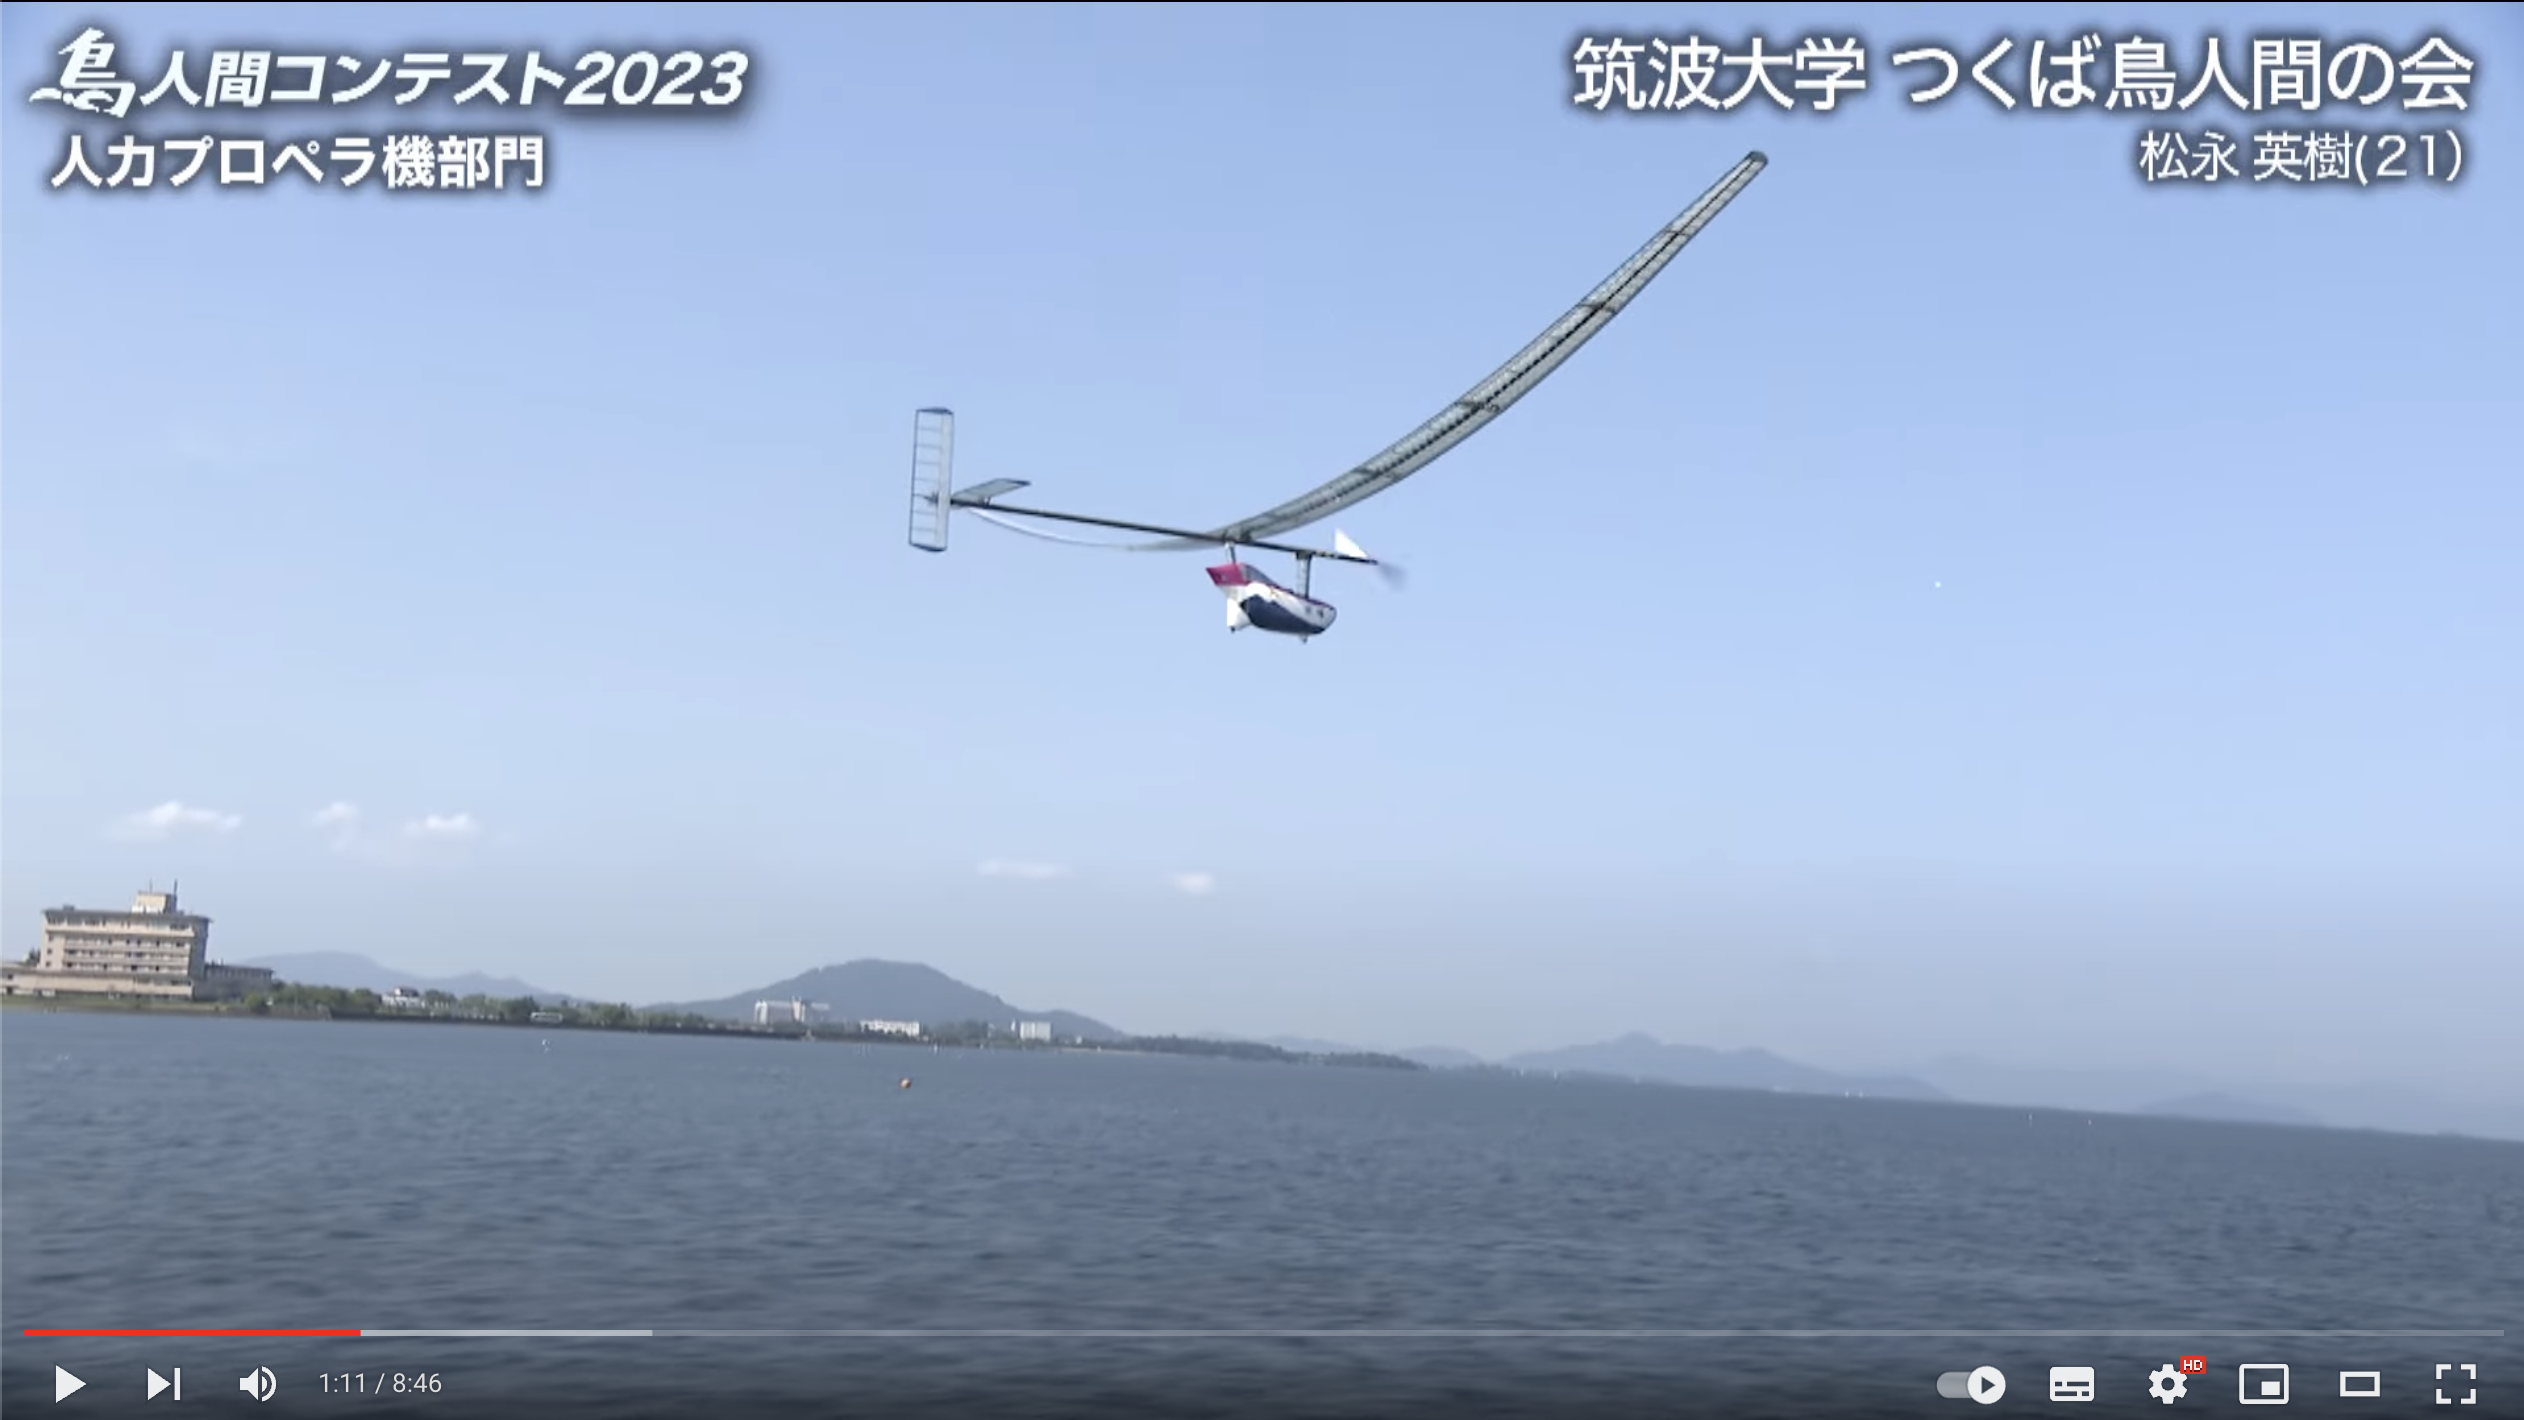
\includegraphics[width=0.7\linewidth]{image/tsukuba0111.png}
    \caption{発進後の高速飛行}
    \label{tsukuba1}
\end{figure}
その後,迎角を下げてさらに高速での飛行を続けます.(図\ref{tsukuba2})
\begin{figure}[H]
    \centering
    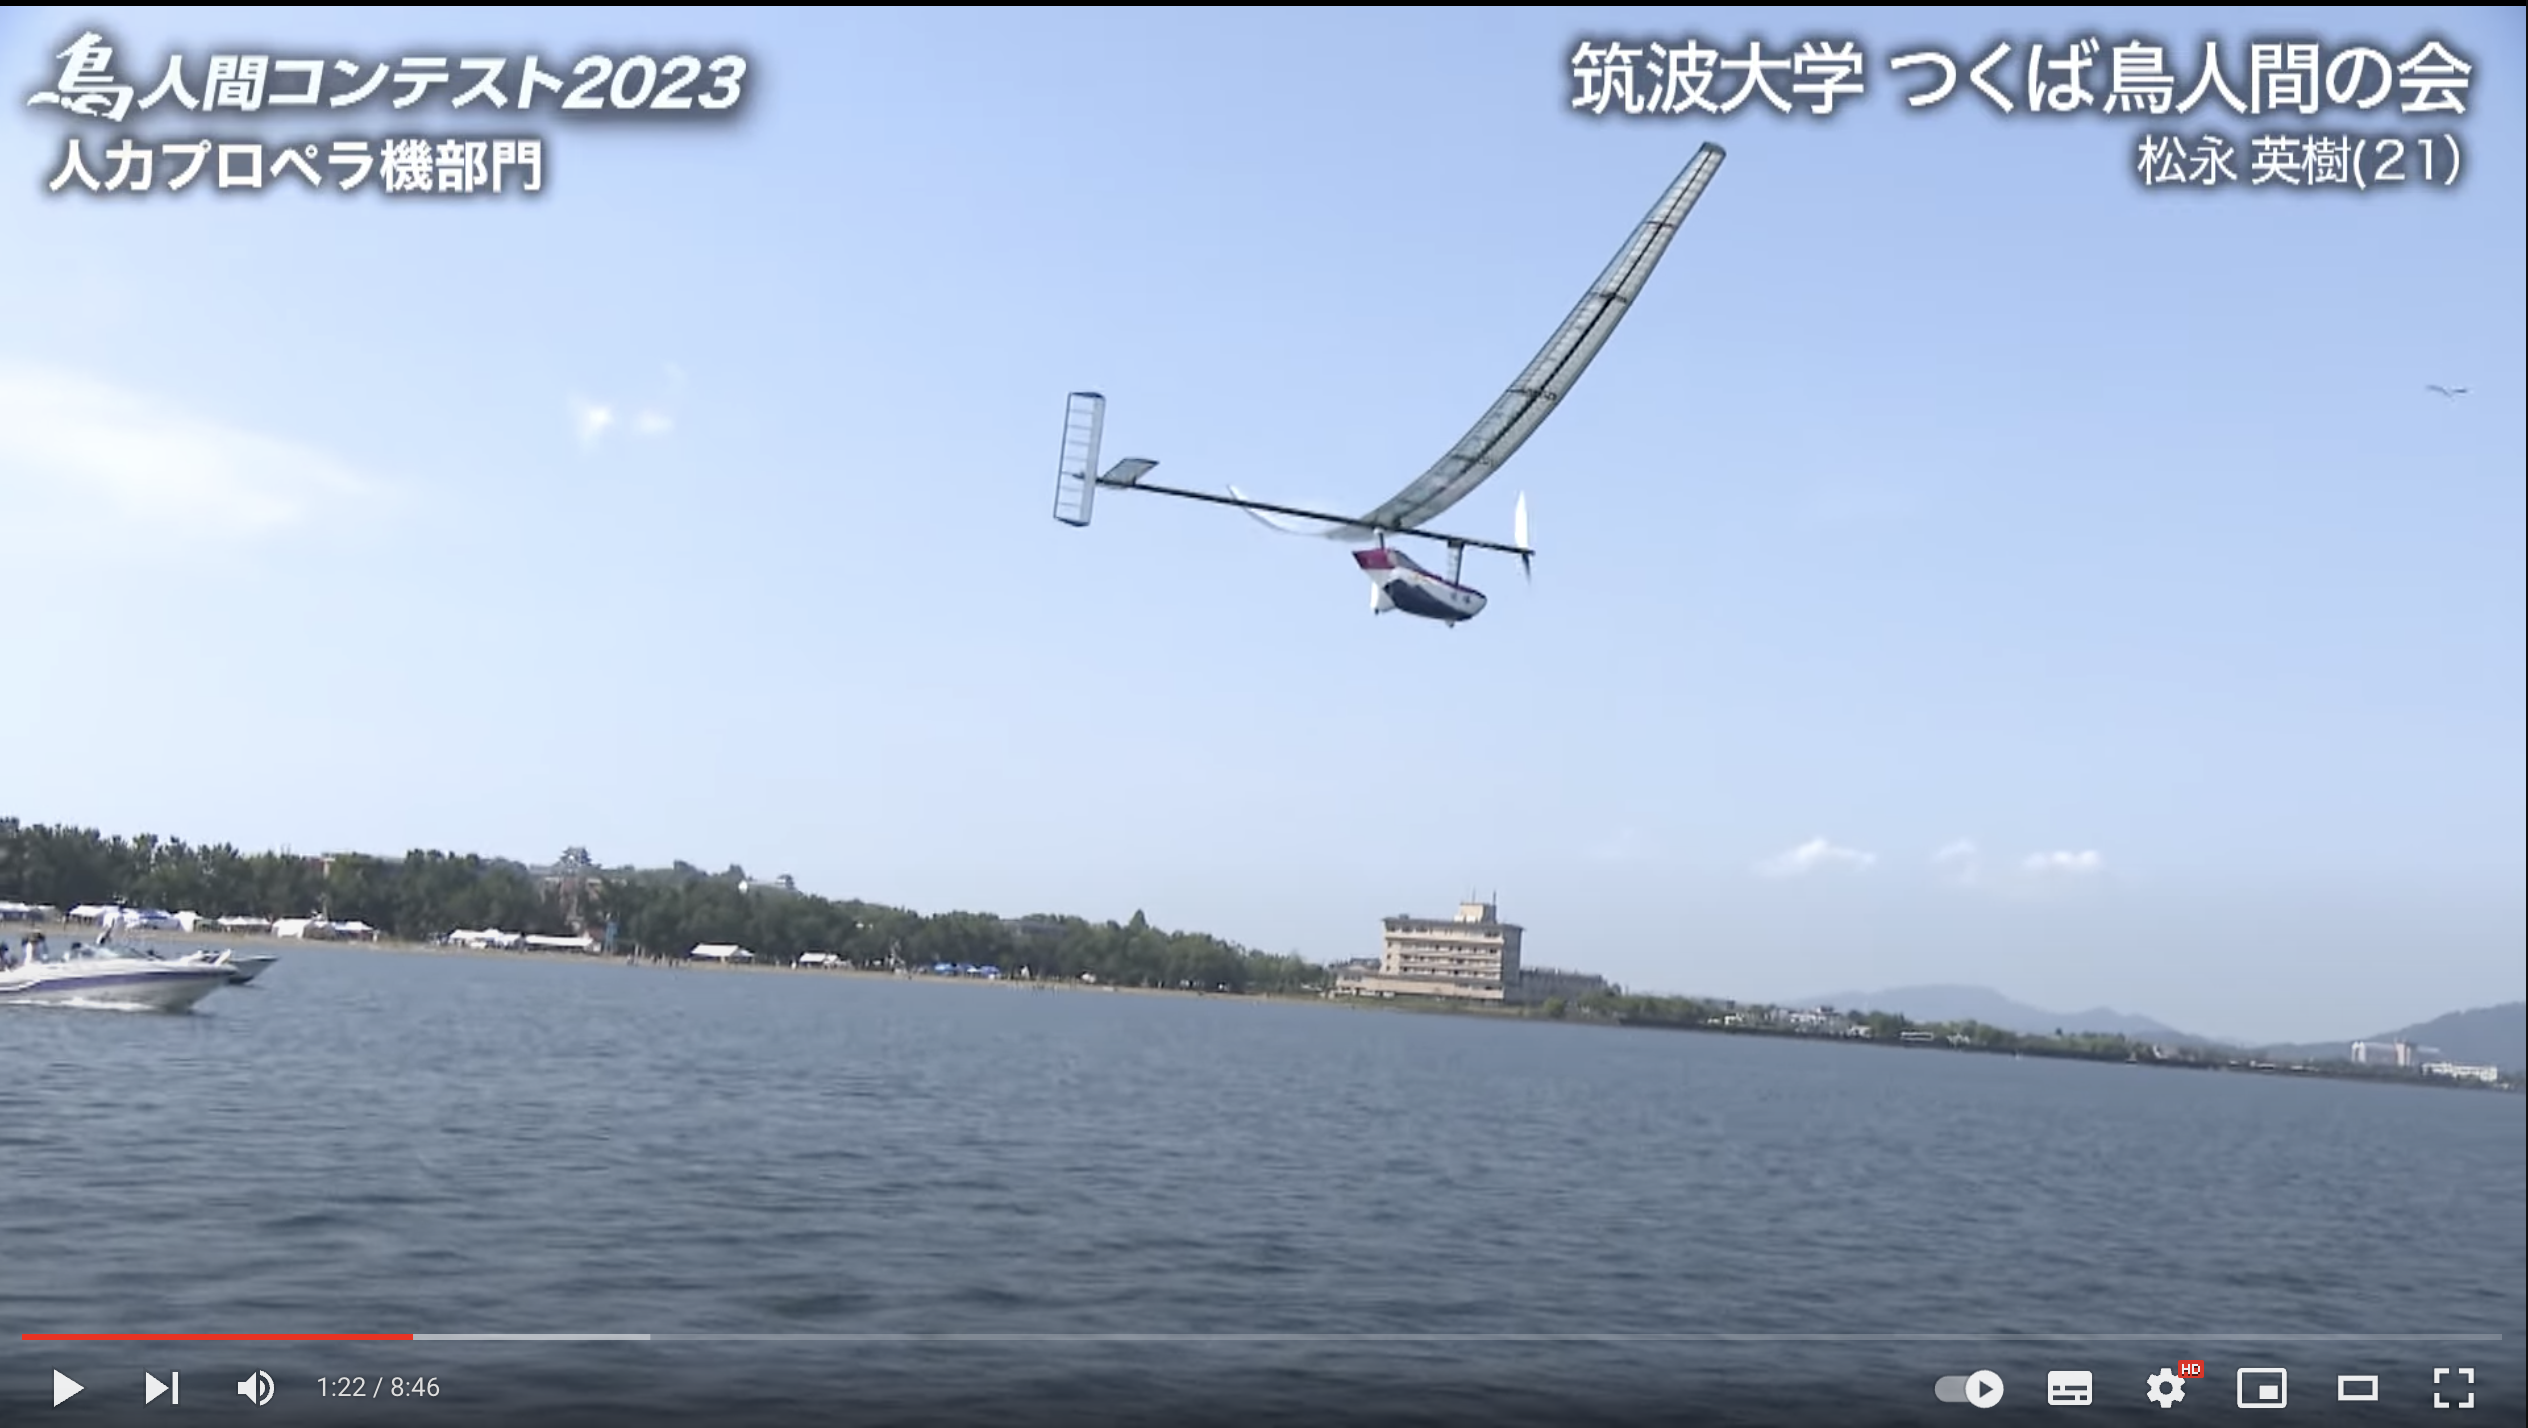
\includegraphics[width=0.7\linewidth]{image/tsukuba0122.png}
    \caption{迎角を下げた様子}
    \label{tsukuba2}
\end{figure}
そして徐々に加速して,機首下げをしながら最終的に翼のねじり下げが生じます.(図\ref{tsukuba3})
\begin{figure}[H]
    \centering
    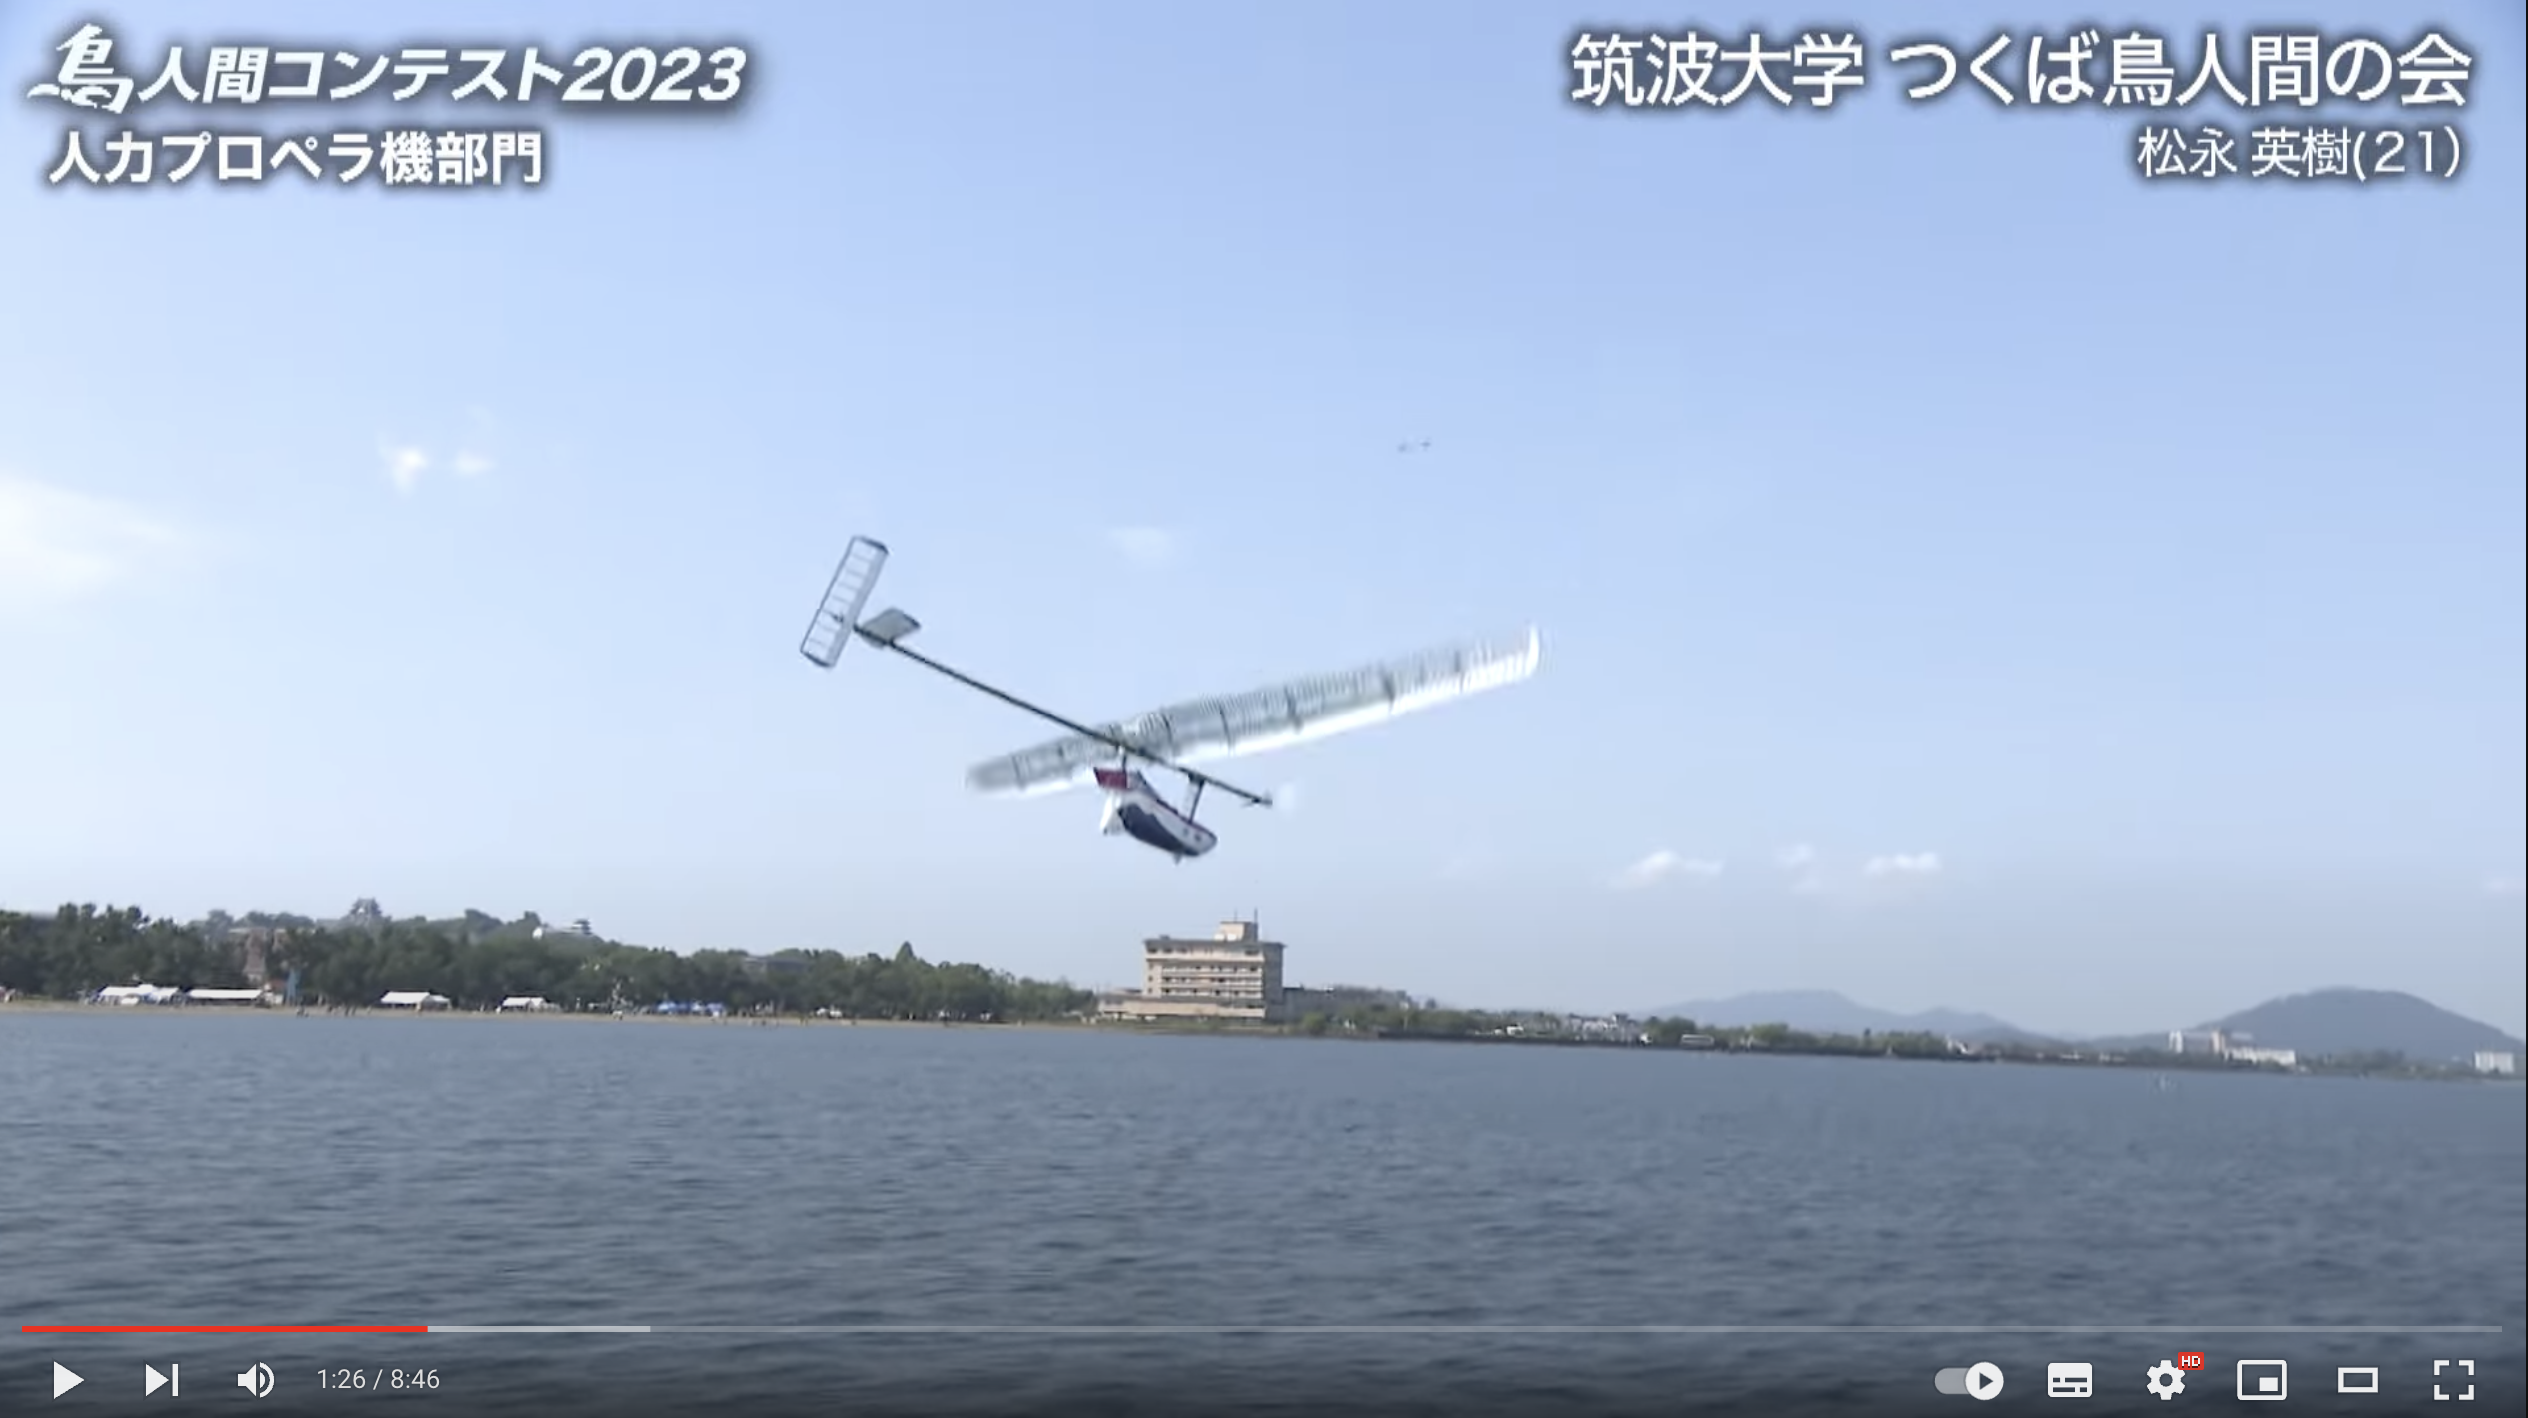
\includegraphics[width=0.7\linewidth]{image/tsukuba0126.png}
    \caption{機首下げとダイバージェンスの発生}
    \label{tsukuba3}
\end{figure}

このように,過剰な速度で飛行した際に翼のねじれが止まらなくなる現象のことをダイバージェンスと呼んでいます.
このダイバージェンスは空力弾性の研究としては既に十分説明されている現象であり,書籍に収録されている内容でもあります\cite{2019}.

しかし,多くの人力飛行機を設計する学生は学部2年生であり,このダイバージェンスの理論的計算を行うには知識不足である場合が多いです.
そのため,本テキストではそのダイバージェンスの理論と具体定な計算方法について説明し,より安全な人力飛行機設計に寄与することを目標としています.

また,今取り扱った筑波大学の例ではフゴイドモードと連成したダイバージェンスモード\cite{takasaki2}\cite{takasaki}による破壊が生じているのではないか,という指摘もあります.
そのため,フゴイドモードと連成したダイバージェンスモードの理論も明らかにし,具体的な計算を行います.
また,その過程で例として示した筑波大学の飛行がどのような状況であったと予想されるか少し触れます.

\newpage

\tableofcontents

\newpage

\section{ダイバージェンス現象の定性的解説}

最初にダイバージェンスの直感的な定義を示します.
\begin{itembox}[l]{ダイバージェンスの直感的定義}
    ダイバージェンスとは,翼のねじれに対して復元力が生じず,翼の捩れが止まらなくなる現象である.
\end{itembox}

この定義を数式で表すためには,翼に生じるねじり力(モーメント)を計算する必要があります.
大まかに空気力と弾性力のモーメントがありますが,まずは翼に生じる空気力によるモーメントを計算します.
座標系は図\ref{chod}の通り前縁を原点に,後縁方向に軸をとります.$h_\mathrm{nw},h_\mathrm{e},X_\mathrm{cp}$はコード長$c$で正規化された空力中心,ねじり中心,風圧中心を示します.
\begin{figure}[H]
    \centering
    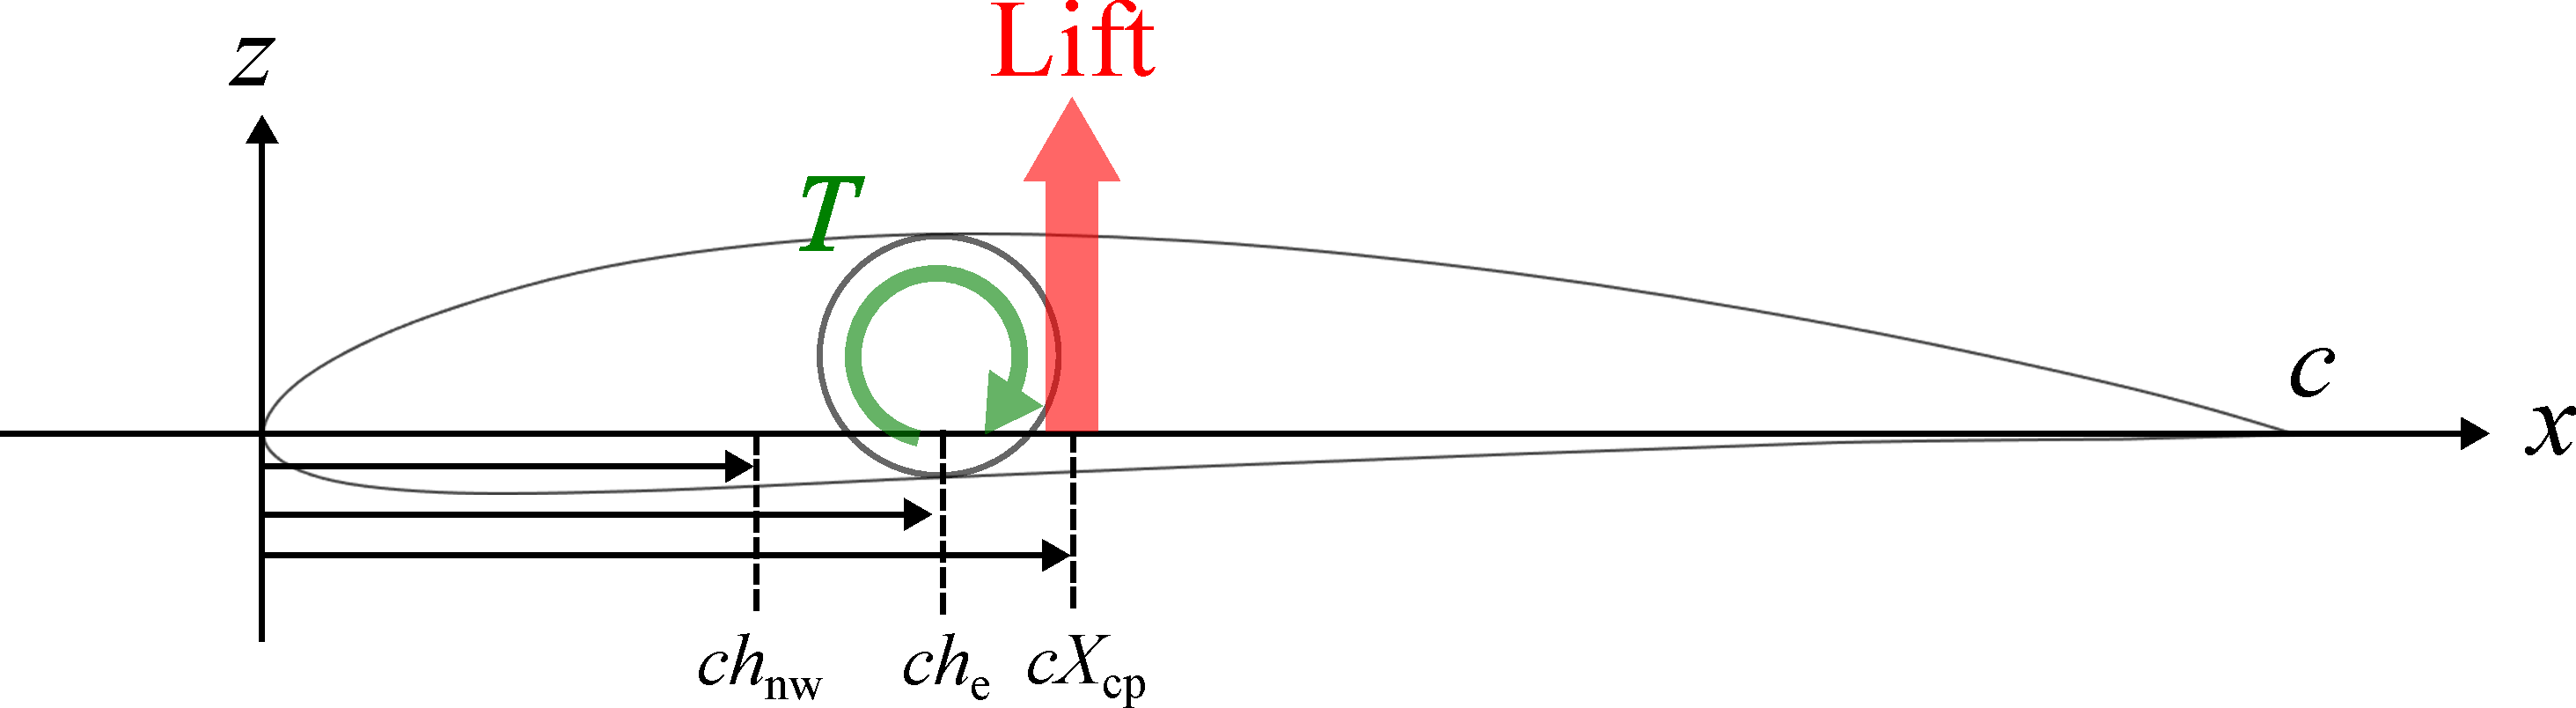
\includegraphics[width=0.7\linewidth]{image/airfoil.pdf}
    \caption{翼断面における代表点の位置関係と力の方向}
    \label{chod}
\end{figure}

最終的には空力中心を使った議論をしたいのですが,まずは風圧中心$cX_\mathrm{cp}$に生じる揚力からモーメントを計算する場合を考えます.
この場合はねじり中心$ch_\mathrm{e}$まわりのねじり上げを正としたモーメントは
\begin{equation}
    T = -\frac{1}{2}\rho U^2 c C_L (cX_\mathrm{cp} - ch_\mathrm{e})
\end{equation}
となります.ねじりモーメントなので,Torsionから$T$をとります.
続いて,空力中心$h_\mathrm{nw}$を使って前縁からの距離を空力中心からの距離に座標変換を行います.
\begin{equation}
    T = -\frac{1}{2}\rho U^2 c C_L ((cX_\mathrm{cp}-ch_\mathrm{nw}) - (ch_\mathrm{e}-ch_\mathrm{nw}))
\end{equation}
これを整理すると空力中心周りのモーメントと,空力中心に生じる空気力によるねじり中心周りのモーメントをに分けることができます.
それを空力中心周りのモーメント係数を使って書き直すと以下の通り書けます.
\begin{equation}
    \begin{split}
        T =& -\frac{1}{2}\rho U^2 c^2 C_L (X_\mathrm{cp}-h_\mathrm{nw}) + \frac{1}{2}\rho U^2 c C_L  (ch_\mathrm{e}-ch_\mathrm{nw}) \\
          =& \frac{1}{2}\rho U^2 c^2 C_m + \frac{1}{2}\rho U^2 c^2 C_L  (h_\mathrm{e}-h_\mathrm{nw})
    \end{split}
\end{equation}
このれが標準的な空気力モーメントの書き方になります.

続いて,ねじれの効果を考えます.このテキストでは翼のねじれ角は$\vartheta$と書きます.
まずは簡単のためにねじれによるモーメントは弾性係数$K$でねじれ角に比例するとします.
また,ねじれることで迎角が変化して揚力係数が変化します.その変化率は揚力傾斜$a=2\pi$として,ねじれる前の揚力係数は$C_{L_0}$とします.
これらの効果を加味して翼に働くねじりモーメントを考えると
\begin{equation}
    T = \frac{1}{2}\rho U^2 c^2 C_m + \frac{1}{2}\rho U^2 c^2 (C_{L_0} + a\vartheta)  (h_\mathrm{e}-h_\mathrm{nw}) - K \vartheta
\end{equation}
となります.これが最も基本的な静的な空力弾性モーメントになります.

翼の断面の慣性モーメントを1とすると,上記のモーメントを使った断面の運動方程式は以下の通りとなります.静的な問題を解くため,慣性モーメントの値は今重要ではありません.
\begin{equation} \label{baseeq}
    \ddot{\vartheta} = \frac{1}{2}\rho U^2 c^2 C_m + \frac{1}{2}\rho U^2 c^2 (C_{L_0} + a\vartheta)  (h_\mathrm{e}-h_\mathrm{nw}) - K \vartheta
\end{equation}
運動の安定性を見る時は,ある釣り合い状態を中心に考えます.そこでその釣り合い状態を計算します.
運動が釣り合っている時は$\ddot{\vartheta}=0$であるため,式(\ref{baseeq})から釣り合い角度$\vartheta_\mathrm{eq}$は,
\begin{equation}
    \vartheta_\mathrm{eq} = \frac{C_m + C_{L_0}(h_\mathrm{e}-h_\mathrm{nw})}{ \frac{K}{\frac{1}{2}\rho U^2 c^2} - a(h_\mathrm{e}-h_\mathrm{nw})}
\end{equation}
となります.この釣り合い角度を用いて$\vartheta = \Delta \vartheta + \vartheta_\mathrm{eq}$として,式(\ref{baseeq})に代入すると以下の釣り合い状態周りの運動方程式が得られます.
\begin{equation} \label{modeq}
    \Delta \ddot{\vartheta} = \frac{1}{2}\rho U^2 c^2 a\Delta \vartheta  (h_\mathrm{e}-h_\mathrm{nw}) - K \Delta \vartheta
\end{equation}

ここで,最初に書いたダイバージェンスの定義を思い出しましょう.
\begin{itembox}[l]{ダイバージェンスの直感的定義}
    ダイバージェンスとは,翼のねじれに対して復元力が生じず,翼の捩れが止まらなくなる現象である.
\end{itembox}
式(\ref{modeq})から考えると,$\vartheta$が増加した時に$\ddot{\vartheta}$が増加する場合,その$\vartheta$の増加を止める術はありません.
これは一つのダイバージェンスの数式的定義として見ることができます.
そのため,数式でダイバージェンスの定義を書き直すと,以下のように書くことができます.
\begin{itembox}[l]{ダイバージェンスの数式での定義}
    ねじれ角の角加速度変化$\Delta \ddot{\vartheta}$について,
    \begin{equation*}
        \frac{\Delta \ddot{\vartheta}}{\Delta \vartheta} > 0
    \end{equation*}
    が成り立つ時翼はダイバージェンスする.特にゼロと等しい場合が安定限界であり,その時の飛行速度$U_\mathrm{div}$をダイバージェンス速度という.
\end{itembox}

今考えている簡単な弾性の場合について,具体的にダイバージェンス速度を計算してみましょう.式(\ref{modeq})を変形すると以下の式が得られます.
\begin{equation}
    \frac{\Delta \ddot{\vartheta}}{\Delta \vartheta} = \frac{1}{2}\rho U^2 c^2 a  (h_\mathrm{e}-h_\mathrm{nw}) - K
\end{equation}
これがゼロと等しい時,$U=U\mathrm{div}$であるため以下の式が成り立ちます.
\begin{equation}\label{Tv}
    \frac{1}{2}\rho U_\mathrm{div}^2 c^2 a  (h_\mathrm{e}-h_\mathrm{nw}) - K = 0
\end{equation}
この式からダイバージェンス速度は
\begin{equation}
    U_\mathrm{div} = \sqrt{\frac{K}{\frac{1}{2}\rho c^2 a  (h_\mathrm{e}-h_\mathrm{nw})}}
\end{equation}
となります.この式からわかることが2点あります.それは
\begin{enumerate}
    \item 空力中心とねじり中心の距離が近いほどダイバージェンス速度は大きい
    \item ねじり弾性力が強いほどダイバージェンス速度は大きい
\end{enumerate}
ということです.特に,空力中心とねじり中心の距離を近くすることは,完全にダイバージェンスの危険性を回避することのできる方法です.
ただし,フラッターやその他動的な空力弾性現象に対しては悪影響が生じうることをご留意ください.

\section{三次元翼のダイバージェンス速度の計算}

前章ではねじり弾性は$K$と単純な比例定数で置いていました.しかし,実際の翼の場合はねじりの弾性力は翼幅方向の微分を含みます.
そのため,次は弾性力を偏微分で書き換えた場合について計算してみます.

まず,対象とする翼を考えます.対象とする範囲は翼の半分で,根元で片持ち固定された梁であると考えます.長さは翼根から翼端まで$L$です.
この時,ねじり剛性$GI_p$を使ってねじり弾性力を以下のように書き換えることができます.翼幅方向を$y$としているため,$y$について微分します.
\begin{equation} \label{gip}
    T = \frac{1}{2}\rho U^2 c^2 C_m + \frac{1}{2}\rho U^2 c^2 (C_{L_0} + a\vartheta)  (h_\mathrm{e}-h_\mathrm{nw}) + GI_p \frac{\partial^2 \vartheta}{\partial y^2}
\end{equation}
この式には付帯条件として以下のねじりの境界条件がつきます.
\begin{align}
    \vartheta(0,t) = 0 \\
    \frac{\partial \vartheta}{\partial y}(L,t) = 0
\end{align}
これは翼根固定端,翼端自由端の条件になります.

式(\ref{gip})をもとにダイバージェンスを計算したいですが,前章まではただの変数であった$\vartheta(t)$が関数である$\vartheta(y,t)$となっています.
そのため,単純に以下の定義を適用することがきません.
\begin{itembox}[l]{ダイバージェンスの数式での定義}
    ねじれ角の角加速度変化$\Delta \ddot{\vartheta}$について,
    \begin{equation*}
        \frac{\Delta \ddot{\vartheta}}{\Delta \vartheta} > 0
    \end{equation*}
    が成り立つ時翼はダイバージェンスする.特にゼロと等しい場合が安定限界であり,その時の飛行速度$U_\mathrm{div}$をダイバージェンス速度という.
\end{itembox}
そのため,システムとしての安定性を見る方法を使う必要があります.この方法を使うにあたっては$\vartheta$が関数のままでは扱いが難しいため,有限要素法を用いた離散化を行います.

\subsection{有限要素法による離散化}

有限要素法はある時間と空間の変数を持つ関数について,その空間分布を節点という代表点で細分化します.
その節点ごとの関数値の時間変化と空間分布を決める関数を考えて,元の関数を表現します.
例えば翼幅方向に等間隔に節点をとる時を考えます.まず,その節点における関数の値を並べたものを列ベクトル$\bm{\vartheta}(t)$と書くことにします.
それに対して各節点の値をもとに元の関数の値を補間する関数(形状関数)$N(y)$を節点の数だけ定義して列ベクトル$\bm{N}(y)$とします.
そしてこの二つを使って元の関数を$\vartheta(y,t) = \bm{N}(y)^\top\bm{\vartheta}(t)$と表現します.
形状関数には色々とパターンがあり,計算の際にもいくつかテクニックがありますが,それについては参考文献とリポジトリにあるプログラムでご確認いただきたいです.
ここでは,ある空間的に広がる関数が空間分布と時間変化部分の積という形に分解できたことが重要ですので,その点だけ覚えてもらえれば問題ないです.

式(\ref{gip})をもとに,有限要素法を用いた離散化を行います.まずは単純に形状関数を使った表現に変更します.
\begin{equation} 
    T = \frac{1}{2}\rho U^2 c^2 C_m + \frac{1}{2}\rho U^2 c^2 (C_{L_0} + a\bm{N}^\top\bm{\vartheta})  (h_\mathrm{e}-h_\mathrm{nw}) + GI_p \frac{\partial^2 \bm{N}^\top}{\partial y^2}\bm{\vartheta}
\end{equation}
この時,空間微分がうまく$\bm{\vartheta}$と分解されていることがわかります.これに左から$\bm{N}$を掛けて,積分します.
\begin{equation} 
    \int_0^L \bm{N} T dy = \int_0^L \left\{ \bm{N} \frac{1}{2}\rho U^2 c^2 C_m +  \frac{1}{2}\rho U^2 c^2 (\bm{N}C_{L_0} + a\bm{N}\bm{N}^\top\bm{\vartheta})  (h_\mathrm{e}-h_\mathrm{nw}) + GI_p \bm{N} \frac{\partial^2 \bm{N}^\top}{\partial y^2}\bm{\vartheta} \right\} dy
\end{equation}
各項について以下のように表記の代用を行います.
\begin{align}
    \bm{T} =& \int_0^L \bm{N} T dy \\
    \bm{T}_\mathrm{25\%} =& \int_0^L \bm{N} \frac{1}{2}\rho U^2 c^2 C_m dy \\
    K_\mathrm{aero} \bm{\vartheta} =& \int_0^L  \frac{1}{2}\rho U^2 c^2 a\bm{N}\bm{N}^\top (h_\mathrm{e}-h_\mathrm{nw}) dy \bm{\vartheta} \\
    K_\mathrm{elastic} \bm{\vartheta} =& \int_0^L GI_p \bm{N} \frac{\partial^2 \bm{N}^\top}{\partial y^2} dy \bm{\vartheta}
\end{align}
特に4つ目の弾性の行列については,部分積分によって簡単にすることができます.
\begin{equation}
    \begin{split}
        K_\mathrm{elastic} =&  \int_0^L GI_p \bm{N} \frac{\partial^2 \bm{N}^\top}{\partial y^2} dy \\
                           =&  \left[ GI_p \bm{N} \frac{\partial \bm{N}^\top}{\partial y} dy  \right]_0^L - \int_0^L GI_p \frac{\partial \bm{N}}{\partial y} \frac{\partial \bm{N}^\top}{\partial y} dy \\
                           =&  - \int_0^L GI_p \frac{\partial \bm{N}}{\partial y} \frac{\partial \bm{N}^\top}{\partial y} dy
    \end{split}
\end{equation}
今回は性質の良い境界条件が使われているため,途中で生じる原始関数はゼロとなります.

以上の結果をもとに式を書き直すと以下の通り線形な方程式になります.
\begin{equation}
    \bm{T} = \bm{T}_\mathrm{25\%} + K_\mathrm{aero} \bm{\vartheta} + K_\mathrm{elastic} \bm{\vartheta}
\end{equation}
$\ddot{\vartheta}$も同様に離散化を行うと離散化した後の運動方程式が得られます.
\begin{align}
    E\ddot{\bm{\vartheta}} =& \bm{T}_\mathrm{25\%} + K_\mathrm{aero} \bm{\vartheta} + K_\mathrm{elastic} \bm{\vartheta} \\
    E =& \int_0^L \bm{N}\bm{N}^\top dy
\end{align}
ここで,$\bm{T}=\bm{0}$となるような$\bm{\vartheta}$を$\bm{\vartheta}_\mathrm{eq}$として,そこからの変化量$\Delta \bm{\vartheta}$について見ることにすると, 
\begin{equation}
    E\Delta\ddot{\bm{\vartheta}} = K_\mathrm{aero} \Delta\bm{\vartheta} + K_\mathrm{elastic} \Delta\bm{\vartheta}
\end{equation}
という平衡状態周りの方程式とできます.

\subsection{行列式・固有値を用いた安定限界の判別}
ところで,以下の微分方程式の一般解を計算する時,どうするでしょうか.
\begin{equation}
    m\ddot{x}(t) = kx(t)
\end{equation}
学部2年生であれば$x(t) = e^{\lambda t}$と置いて$\lambda$を求めることで計算すると思います.
例えば今回の場合$\lambda^2 = k/m$となるため,解は次の3つが考えられます.
\begin{align*}
    k/m < 0の場合:& \ x(t) = A\sin\sqrt{k/m}t + B\cos\sqrt{k/m}t \\
    k/m = 0の場合:& \ x(t) = At + B \\
    k/m > 0の場合:& \ x(t) = Ae^{\sqrt{k/m}t} + Be^{-\sqrt{k/m}t}
\end{align*}
この時,$m$は正であるため$A,B$によらず解が発散しないのは$k < 0$の時のみで,安定の限界にあるのは$k=0 \Leftrightarrow \lambda = 0$の時になります.
そのため,安定限界を調べる場合は$\lambda=0$の条件下で計算を行い,$k=0$に相当する条件を見つければ良いことになります.

では,以下の式について同様のことを考えてみましょう.
\begin{equation}
    E\Delta\ddot{\bm{\vartheta}} = K_\mathrm{aero} \Delta\bm{\vartheta} + K_\mathrm{elastic} \Delta\bm{\vartheta}
\end{equation}
$\bm{C}$をゼロでないベクトルとして$\Delta\bm{\vartheta} = \bm{C}e^{\lambda t}$とすると,
\begin{equation}
    \left\{ E\lambda^2 - (K_\mathrm{aero} + K_\mathrm{elastic}) \right\}\bm{C}e^{\lambda t} = \bm{0}
\end{equation}
となります.ここで,安定が限界となる条件は先の例題と同様に$\lambda = 0$であるため,その条件を代入すると以下の式となります.
\begin{equation}
    (K_\mathrm{aero} + K_\mathrm{elastic})\bm{C}e^{\lambda t} = \bm{0}
\end{equation}
この式は$\bm{C}e^{\lambda t} \neq 0$である時にも成り立つため,$K_\mathrm{aero} + K_\mathrm{elastic}$の行列式はゼロであると考えられます.
そのため,この行列式がゼロであることが安定限界の条件になります.
また,行列式がゼロであることは,その行列の固有値には少なくとも一つのゼロが含まれることと同値であるため,この行列の固有値を見ることでも安定性を判別することができます.

最終的にまとめて書くと,以下の条件を満たす時に安定限界であると言えます.
\begin{itembox}[l]{三次元翼のダイバージェンスの安定限界の近似}
    有限要素法から得られた空力ねじりモーメント係数行列$K_\mathrm{aero}$,弾性ねじりモーメント係数行列$K_\mathrm{elastic}$の和について,
    \begin{enumerate}
        \item 行列式がゼロである時
        \item 固有値に少なくとも一つのゼロが含まれる時
    \end{enumerate}
    のどちらかが成り立つ時,ダイバージェンスの安定限界である.
\end{itembox}


\subsection{具体的な計算例}

具体的な翼,例えばある人力飛行機のパラメータで計算してみましょう.
この人力飛行機は片持ち翼で,桁位置は定常飛行時の風圧中心に合わせています.桁直径は根本は100mm,翼端は40mmで40tプリプレグを$\pm$45度1組入れています.
スパンの半分である$L$は14.7 mとしています.
分割数は150分割で,形状関数は一次バー要素として計算します.
その結果が以下の図\ref{eigen1}です.

\begin{figure}[H]
    \centering
    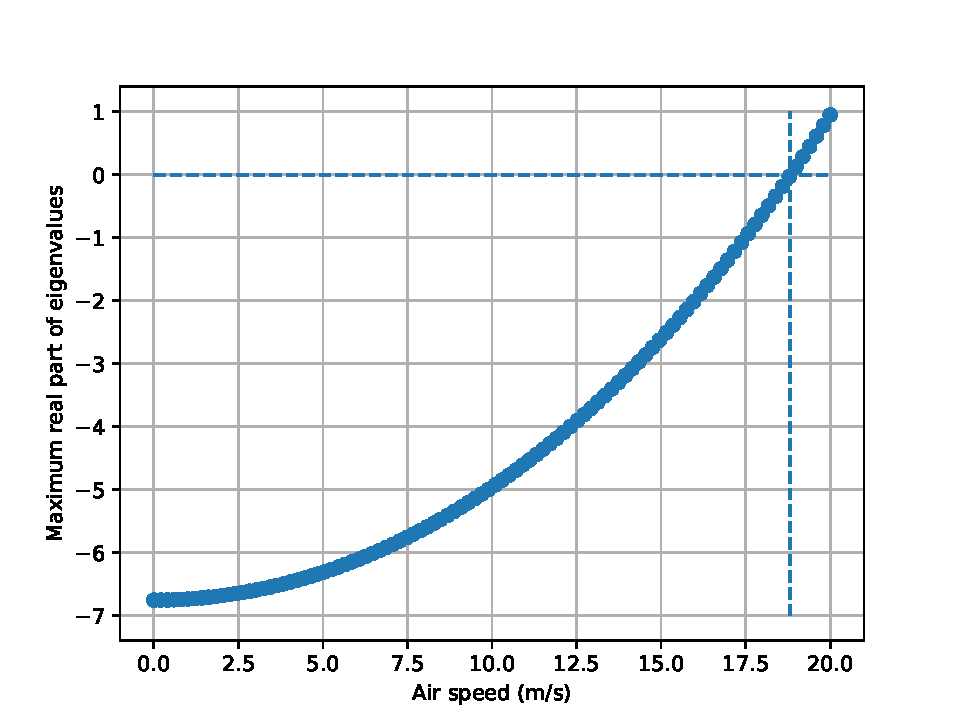
\includegraphics[width=0.8\linewidth]{image/Eigenvalues_of_divergence.pdf}
    \caption{速度ごとの係数行列の固有値実部の最大値}
    \label{eigen1}
\end{figure}

この結果プロットは横軸に表す飛行速度において,計算の結果得られた150個の固有値の実部のうち一番大きなものをプロットしています.
一般に分解の結果得られる固有値は複素数ですが,今回は係数行列が実対称行列であるため得られる固有値は全て実数になります.
そこで,実部のみを提示しています.
最初はすべての固有値が負ですが,おおよそ18.8 m/sにおいて最大の固有値がゼロ,つまり安定限界になっていることがわかります.
そのため,この人力飛行機のダイバージェンス速度は18.8 m/sであると考えられます.

\section{フゴイドモードと連成するダイバージェンス現象}

ここまでに通常のダイバージェンスについて計算を行いました.
しかし,フゴイドモードとダイバージェンスが相互に影響することでさらに安定性が低下する事例があると指摘されています\cite{takasaki}.
そこで,本章ではこれについて参考文献とは別の方針で具体的に計算を行います.

まずはフゴイドモードの運動方程式を示します.
\begin{align} 
    \dot{u} - X_u u + g \theta = 0\\
    -U\dot{\theta} - Z_u u = 0
\end{align}
これは航空機力学入門(白本)\cite{sirohon}を参考に,全機質量が1の場合を考えています.先にも言ったように,静的な問題については慣性の値はゼロでない何でも良いので1としています.
ここに書かれている$u,\theta$は機体の機体固定座標系で見た前進飛行速度,ピッチ角であり,$U$は釣り合い時の$u$のです.
$X_u,Z_u$は機体固定座標系での並進空気力$X,Z$を$u$によって偏微分していることを意味します.
$X$はこの後消えるため無視しますが,$Z$については以下のように定義します.航空機では下向きが正なので揚力は負の値です.
\begin{equation}
    Z = -\int_{-L}^L \frac{1}{2}\rho U^2 c (C_{L_0} + a\vartheta) dy
\end{equation}
フゴイドモードの仮定により迎角$\alpha$による影響は含みません.その代わりにねじれ角$\vartheta$の影響があります.

フゴイドモードに加えてねじれの釣り合いとねじれの影響を追加すると以下の通りとなります.
\begin{align} 
    \dot{u} - X_u u + g \theta = X_\vartheta \vartheta \label{X}\\
    -U\dot{\theta} - Z_u u = Z_\vartheta \vartheta \label{Z} \\
    \ddot{\vartheta} = T_u u + T_\vartheta \vartheta \label{vt}
\end{align}
ここに現れる$T$は式(\ref{gip})を$U \rightarrow u$に調整したもので,以下の通りとなります.
\begin{equation}
    T = \frac{1}{2}\rho u^2 c^2 C_m + \frac{1}{2}\rho u^2 c^2 (C_{L_0} + a\vartheta)  (h_\mathrm{e}-h_\mathrm{nw}) + GI_p \frac{\partial^2 \vartheta}{\partial y^2}
\end{equation}
ここで式(\ref{X})を時間微分して式(\ref{Z})を代入すると次の式が得られます.
\begin{align}
    \ddot{u} = X_u \dot{u} + X_\vartheta \dot{\vartheta} + \frac{g}{U} (Z_u u + Z_\vartheta \vartheta) 
\end{align}
今回取り扱う問題は静的な問題のみを取り扱うため,$\dot{u},\dot{\vartheta}$の影響はないものとします.すると式(\ref{vt})と合わせて以下の形に簡単になります.
\begin{align}
    \ddot{u} =&   \frac{g}{U}Z_u u + \frac{g}{U}Z_\vartheta \vartheta \\
    \ddot{\vartheta} =& T_u u + T_\vartheta \vartheta
\end{align}

この式に対して行列式を使った安定限界の判別を行います.前章と同様に指数関数を代入すると以下の式が得られます.
\begin{equation}
    \left\{
    \begin{bmatrix}
        1 & 0 \\
        0 & 1
    \end{bmatrix}
    \lambda^2
    -
    \begin{bmatrix}
        \frac{g}{U}Z_u & \frac{g}{U}Z_\vartheta \\
        T_u & T_\vartheta
    \end{bmatrix}
    \right\}
    \bm{C}e^{\lambda t}
    =
    \bm{0}
\end{equation}
以上の式において$\lambda=0$とした時の行列式がゼロになる条件を考えることで,フゴイド連成ダイバージェンス速度$U_\mathrm{pdiv}$を求めることができます.
\begin{equation}
    \left|
    \begin{matrix}
        \frac{g}{U_\mathrm{pdiv}}Z_u & \frac{g}{U_\mathrm{pdiv}}Z_\vartheta \\
        T_u & T_\vartheta
    \end{matrix}
    \right|
    =0
\end{equation}
\begin{equation}\label{phudiv2}
    \frac{g}{U_\mathrm{pdiv}} (Z_u T_\vartheta - Z_\vartheta T_u ) = 0
\end{equation}
以上の計算から,フゴイド連成ダイバージェンス速度の時
\begin{equation}
    Z_u T_\vartheta - Z_\vartheta T_u  = 0
\end{equation}
が成り立つことがわかります.
特に,これを変形した以下の形で以降の議論に使用します.
\begin{align}\label{phudiv}
    T_\vartheta = \frac{Z_\vartheta T_u}{Z_u}
\end{align}
また各値は具体的には以下の通りとなります.ねじり弾性については簡単のために定数$K$としています.
\begin{align}
    T_\vartheta =& \int_{-L}^{L} \left\{ \frac{1}{2}\rho U_\mathrm{pdiv}^2 c^2 a  (h_\mathrm{e}-h_\mathrm{nw}) - K \right\} dy \label{Tv1} \\
    Z_\vartheta =& -\int_{-L}^L \frac{1}{2}\rho U_\mathrm{pdiv}^2 c a dy \\
    T_u =& \int_{-L}^L \rho U_\mathrm{pdiv} c^2 \left\{ C_m +  (C_{L_0} + a\vartheta_\mathrm{eq})  (h_\mathrm{e}-h_\mathrm{nw}) \right\} dy \\
    Z_u =& -\int_{-L}^L \rho U_\mathrm{pdiv} c (C_{L_0} + a\vartheta_\mathrm{eq}) dy
\end{align}
式(\ref{Tv1})と式(\ref{Tv})を比較すると,この$T_\vartheta$はダイバージェンスの安定限界を調べるために用いたものと同じであることがわかります.
そのため,式(\ref{phudiv})の右辺が正である場合は$U_\mathrm{pdiv}>U_\mathrm{div}$となりますが,先にダイバージェンス速度$U_\mathrm{div}$になるためダイバージェンスで破壊します.

また,式(\ref{phudiv})について右辺の値が負である場合は$U_\mathrm{pdiv} < U_\mathrm{div}$となります.この右辺の正負は$T_u$によって決まります.
$Z_u,Z_\vartheta$は常に負であることが容易にわかりますが,$T_u$については$C_m +  (C_{L_0} + a\vartheta_\mathrm{eq})  (h_\mathrm{e}-h_\mathrm{nw})$によって正負が反転します.
この正負の反転は桁位置$h_\mathrm{e}$と風圧中心$X_\mathrm{cp}$の前後関係によって決まります.

$T$について,当初提示した表現を見てみましょう.
\begin{equation}
    T = -\frac{1}{2}\rho u^2 c C_L (cX_\mathrm{cp} - ch_\mathrm{e})
\end{equation}
この式を速度$u$について微分すると以下の式が得られます.
\begin{equation}
    T_u = -\rho U c C_L (cX_\mathrm{cp} - ch_\mathrm{e})
\end{equation}
この式を見ると,風圧中心と桁位置の前後関係が$T_u$の正負に大きな影響を与えることがわかります.
それを加味して考えると,ダイバージェンスとフゴイド連成ダイバージェンスの条件分岐は以下の通りとなります.
\begin{enumerate}
    \item $h_\mathrm{e} > X_\mathrm{cp}$の時$T_u>0$となり,$\frac{Z_\vartheta T_u}{Z_u} > 0$となる.この時ダイバージェンス速度で破壊する.
    \item $h_\mathrm{e} < X_\mathrm{cp}$の時$T_u<0$となり,$\frac{Z_\vartheta T_u}{Z_u} < 0$となる.この時フゴイド連成ダイバージェンス速度で破壊する.
\end{enumerate}

まず1の場合については,第2章と同様にねじり剛性を上げるか,桁位置を前に寄せることが対策として考えられます.ただし,桁位置が風圧中心より前に行くとフゴイド連成のダイバージェンスに切り替わります.

2の場合については,$c$以外はスパン方向に一定であると仮定して,平均空力翼弦を$\bar{c}$として式(\ref{phudiv2})を速度について整理すると
\begin{equation}
    U_\mathrm{pdiv} = \sqrt{ \frac{K}{\frac{1}{2}\rho S\bar{c}a(h_\mathrm{e}-h_\mathrm{nw})} } \sqrt{\frac{(C_{L_0}+a\vartheta_\mathrm{eq})(h_\mathrm{e}-h_\mathrm{nw})}{-C_m}}
\end{equation}
となります.ここで,左辺の一個目の平方根は$U_\mathrm{div}$を長手方向に積分したものと一致するため,$U_\mathrm{div}$と書きます.
\begin{equation} \label{pdiv}
    U_\mathrm{pdiv} = U_\mathrm{div} \sqrt{\frac{(C_{L_0}+a\vartheta_\mathrm{eq})(h_\mathrm{e}-h_\mathrm{nw})}{-C_m}}
\end{equation}
桁位置は風圧中心より前なので,$T_u<0$であり,$|C_m| >  |(C_{L_0} + a\vartheta_\mathrm{eq})  (h_\mathrm{e}-h_\mathrm{nw})|$となります.
そのため,式に残った平方根は1より小さく,常に$U_\mathrm{pdiv} < U_\mathrm{div}$が成り立ちます.
結果として$U_\mathrm{pdiv}$の上限は$U_\mathrm{div}$となります.
そして$U_\mathrm{pdiv}$を上限に近づけるには,できる限り$C_m$を小さくすると良いことがわかります.

以上の結果から,フゴイド連成ダイバージェンスに対する定性的な対策として以下の2つが考えられます.
\begin{enumerate}
    \item 桁のねじり剛性を大きくすることで,フゴイド連成ダイバージェンス速度の上限を上げる.
    \item $|C_m|$の小さな翼型を使うことで,上限の範囲内でフゴイド連成ダイバージェンス速度上げる.
\end{enumerate}
また,$h_\mathrm{e}-h_\mathrm{nw}$を変更しても分母分子で相殺するため,$U_\mathrm{pdiv}$には特に影響はありません.
そのため,桁位置については任意に置いても良いという考え方もできます.
しかし,これについては空力弾性的な動特性に対する影響が私にはわからないため,あまり従来の位置を外さないようにした方が無難と思います.
また,構造の構成上非常に不利になることも考えられます.\textbf{桁位置による不安定モードの調整は基本的に全くもって推奨できません.}ねじり剛性か$C_m$での根本的な解決を推奨します.

\subsection{三次元翼における計算}

ここまでで定性的な結果を示しましたが,実際にフゴイド連成ダイバージェンス速度を計算するには弾性の偏微分に対処する必要があります.
前章では有限要素法を用いて計算を行いましたが,本問題においては有限要素法を用いて計算を行うと数値計算上の問題が生じます.
これは,現象としては同じ重みであるフゴイドとねじれについて,それぞれ表現のために必要な要素数が1次元と150次元と大きな差があるため,フゴイドが過小に評価されてしまうからであると考えています.

そこで,離散化ではなくモデルの低次元化を用いることにしました.モデルの低次元化はモード法というものを用います.
このモード法はねじりの境界条件を満たす空間分布に関する関数(モード)$\phi(y)$を用意して,実際の運動$\vartheta$を$\phi$と時間変化するモードの重み$w(t)$を用いて$\vartheta=\phi w$と近似します.
このモードは複数使っても良いですが,今回は簡単のために1つのみとします.実際に計算すると一つでも問題ありません.
モードの計算方法についてはプログラムをご覧ください.

モード法を用いると,$T_\vartheta,Z_\vartheta,T_u,Z_u$それぞれは以下の通りとなります.
\begin{align}
    T_\vartheta =& \int_{-L}^{L} \left\{ \frac{1}{2}\rho U_\mathrm{pdiv}^2 c^2 a \phi  (h_\mathrm{e}-h_\mathrm{nw}) - GI_p\left( \frac{\partial \phi}{\partial y} \right)^2 \right\} dy \\
    Z_\vartheta =& -\int_{-L}^L \frac{1}{2}\rho U_\mathrm{pdiv}^2 c a \phi dy \\
    T_u =& \int_{-L}^L \rho U_\mathrm{pdiv} c^2 \left\{ C_m +  (C_{L_0} + a\phi w_\mathrm{eq})  (h_\mathrm{e}-h_\mathrm{nw}) \right\} dy \\
    Z_u =& -\int_{-L}^L \rho U_\mathrm{pdiv} c (C_{L_0} + a\phi w_\mathrm{eq}) dy
\end{align}
関数$\phi$の積分であるので,得られる結果は単純なスカラーになります.これらからなる復元力行列
\begin{equation}
    \begin{bmatrix}
        \frac{g}{U}Z_u & \frac{g}{U}Z_\vartheta \\
        T_u & T_\vartheta
    \end{bmatrix}
\end{equation}
の行列式・固有値を見ることで計算することができます.

\subsection{具体的な計算例}

実際の三次元的な翼に対して,モード抽出ののちにフゴイド連成ダイバージェンス速度の計算を行います.
先ほどダイバージェンスの計算に使用したパラメータでモードの抽出を行うと,図\ref{mode}が得られます.
\begin{figure}[H]
    \centering
    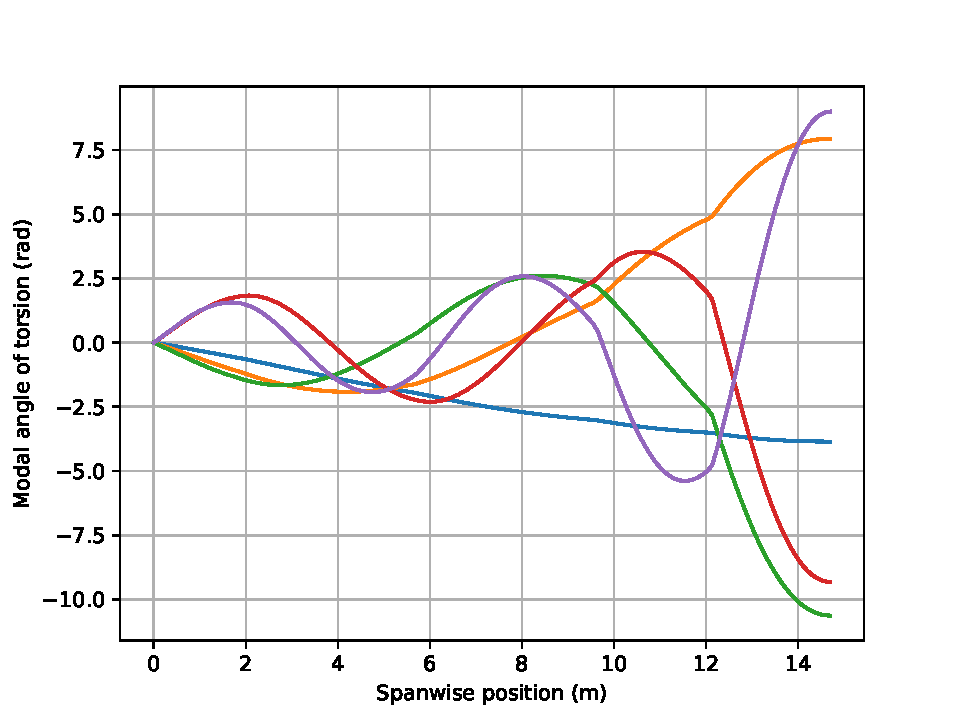
\includegraphics[width=0.7\linewidth]{image/theta_mode.pdf}
    \caption{片翼分のねじり弾性モード}
    \label{mode}
\end{figure}
図\ref{mode}には固有角振動数の小さなものから順に5つのモードを示しています.特に青色が今回計算に用いた最も緩慢なモードです.

これに基づいて$C_m$の値が$0,-0.1,-0.2,-0.3$の4ケースを計算した結果が図\ref{eigen2}になります.
$C_m=-0.3$は非現実的な極端な事例ですが,計算上の差がわかりやすくなるためケースとして含めています.
\begin{figure}[H]
    \centering
    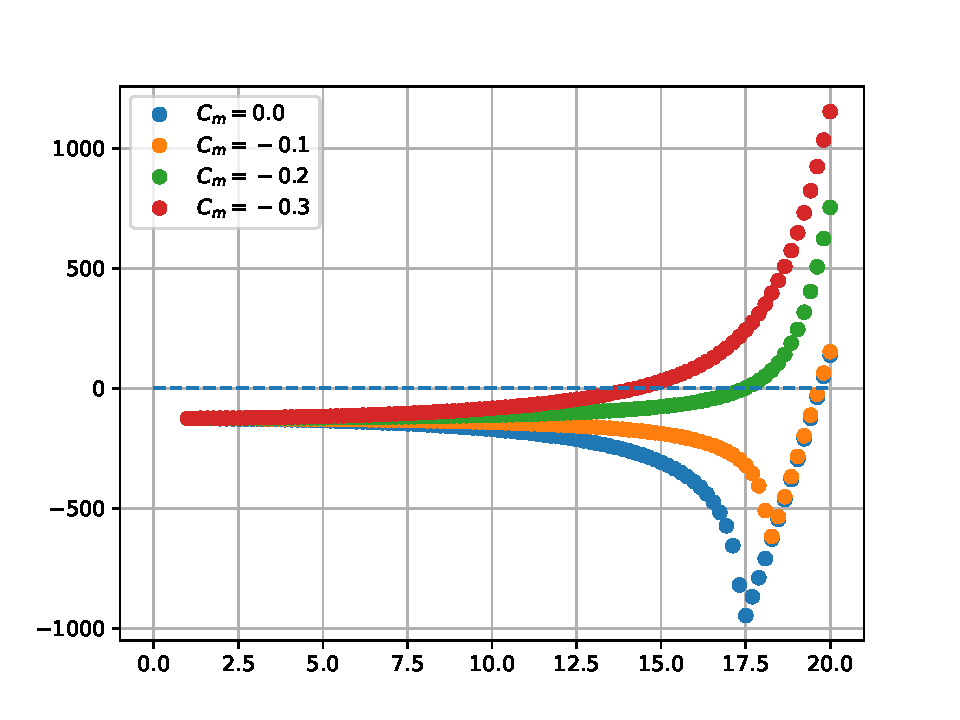
\includegraphics[width=0.7\linewidth]{image/eigenplot.pdf}
    \caption{速度ごとの固有値実部の最大値}
    \label{eigen2}
\end{figure}
このように,$C_m$がある程度の値を超えるまでは通常のダイバージェンスと同じ程度の速度で安定限界になり,
それ以降はフゴイド連成のダイバージェンス速度で安定限界になることがわかります.
今回は$C_{L_0}=1.0$に固定していますので,$C_m$の変化量は風圧中心の位置の変化量に相当します.
そのため,$C_m$に応じて風圧中心が後ろに移動し,ある$C_m$において桁位置と風圧中心の位置関係が逆転して,安定限界の飛行速度が下がったと見られます.

この計算においては$C_{L_0}=1.0$と固定しましたが,実際の飛行状況によっては$C_{L_0}$の値は変化します.
例えば水平飛行を想定して揚力一定の条件を課すと,飛行速度が増加した際に釣り合いの揚力係数は減少するべきです.

そこで,$C_m=-0.1$かつ飛行速度8.5 m/sで揚力係数1.0で釣り合う場合において,飛行速度が変動しても揚力が一定になるように揚力係数を変更して計算を行いました.
その例が図\ref{eigen3}です.失速のことを考慮して,揚力係数は最大1.3までとしています.
\begin{figure}[H]
    \centering
    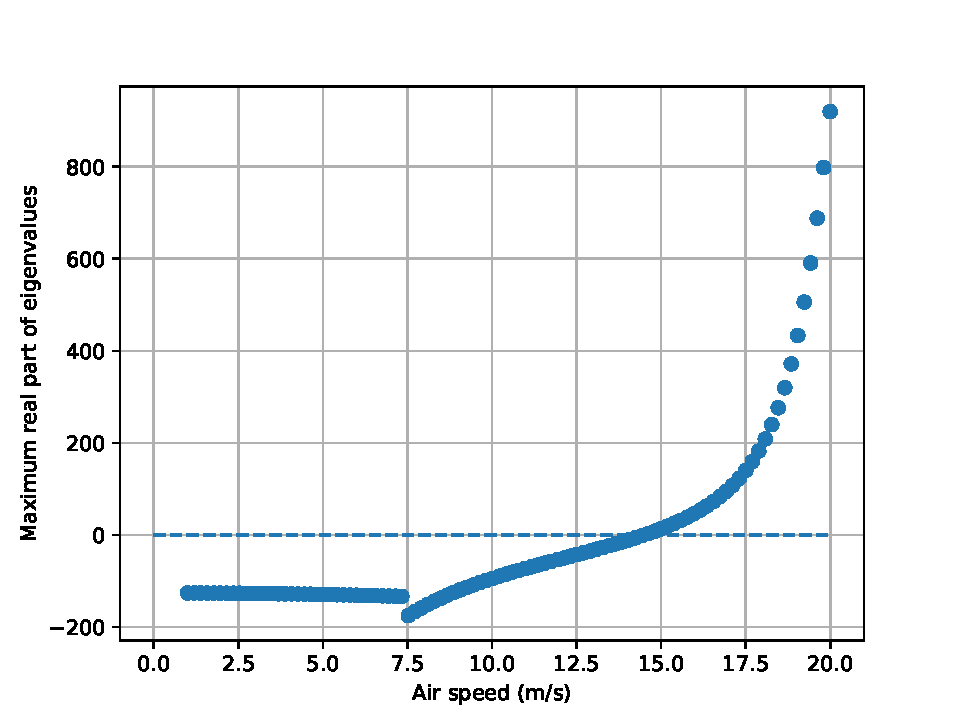
\includegraphics[width=0.7\linewidth]{image/Eigenvalues_of_phugoid-divergence-modal-varCL-0.1.pdf}
    \caption{揚力一定での速度ごとの固有値実部の最大値}
    \label{eigen3}
\end{figure}
$C_m=-0.1$の場合は図\ref{eigen2}ではダイバージェンス速度で安定限界となっていましたが,図\ref{eigen3}ではダイバージェンス速度未満で安定限界となっていることがわかります.
この計算例の定性的な理解としては,高速飛行でも揚力を一定に保つために$C_{L_0}$が減少したため風圧中心が後退し,$U_\mathrm{div}$より遅い速度で風圧中心の位置が桁位置より後ろになってフゴイド連成のダーバージェンス速度で安定限界になったと考えられます.

この事象が現れているであろう例としては,1章において示した筑波大学の例があります.
筑波大学の主翼設計は桁位置と風圧中心を合わせる方針と見られるため,定常飛行状態で速度が大きくなった場合はダイバージェンスで破壊します.
しかし,大会では途中で機首下げにしたことで$C_{L_0}$が減少し,図\ref{tsukuba2}の状態では風圧中心が桁より後ろになったと考えられます.
この場合は安定限界はフゴイド連成のダイバージェンスになるため,映像のような機首下げ運動と同時にねじれが進行するような運動を生じたのではないかと考えられます.

\section{おわりに}

本テキストではダイバージェンスとフゴイド連成ダイバージェンスについて理論と実際の計算例を示しました.
本テキストの図表などを計算するために用いたプログラムなどはgithubリポジトリ\cite{git}において公開しています.
使用にあたってのライセンスはMITであり,ほとんどすべての使用方法が許容されていますが,同時に使用に付随して発生する問題に対する保証もありません.
ただし,この計算結果のみをもとに十分な検討なく限界に近い設計を行うなどの安全に資さない使い方は避けていただきたいです.

\begin{thebibliography}{99}
    \bibitem{2019} 中道二郎,玉山雅人,児玉智,「航空宇宙工学テキストシリーズ 空力弾性学」,日本航空宇宙学会,2019.
    \bibitem{takasaki2} \UTF{9AD9}嵜浩一,「人力飛行機/高高度無人機特有の飛行力学/空力弾性の連成に関する考察」,第23回スカイスポーツシンポジウム,2017,Available: \url{http://flightlogbook.cocolog-nifty.com/logbook/files/23rdSSS_presentation_20171205_part0.pdf} (accessed Mar. 2024).
    \bibitem{takasaki} \UTF{9AD9}嵜浩一,「高高度無人機・人力飛行機のヒュゴイドモード/空力弾性連成運動に対する翼端後退角の効果について」,第27回スカイスポーツシンポジウム,2022,[Online],Available: \url{http://flightlogbook.cocolog-nifty.com/logbook/2022/12/post-ffe4a8.html} (accessed Feb. 2024).
    \bibitem{sirohon} 加藤寛一郎,大屋昭男,柄沢研治,「航空機力学入門」,東京大学出版会,1982.
    \bibitem{git} 中村亮介,「Phugoid-divergence」,FlyingSheeps Github repositories,\url{https://github.com/FlyingSheeps/Phugoid-divergence/tree/main}, (accessed Feb. 2024).
\end{thebibliography}

\end{document}
